%%%%%%%%%%%%%%%%%%%%%%%%%%%%%%%%%%%%%%%%%%%%%%%%%%%%%%%%%%%%%%%%%%%%%%%%%%%%%%%%%%%
% Team:
% EagleUnit
% Members: 
%  I-Chei, Chinweze, Jones, Ray, Hunry, Piyarul, Tim
% Relative files:
% 
% Note:    
% 
%%%%%%%%%%%%%%%%%%%%%%%%%%%%%%%%%%%%%%%%%%%%%%%%%%%%%%%%%%%%%%%%%%%%%%%%%%%%%%%%%%%

\subsection{XML metadata structure}
\label{sec:abs}
Our responsibility is to build a metadata schema which contains all information in a PDF and then program it in an XML structure. This article presents an overview of metadata standards related to our responsibility. We reviewed a number of metadata schemas in use today, including MODS, METS, METS+MODS+PREMIS, MARC21, MARC XML, Dublin Core showing the overview, pros, and cons of each schema. Finally, by examining the characteristics and unique features of these metadata schemas, we were able to rank them and suggest the optimum standard to be used to accomplish our responsibility.\\

Metadata is defined as "data about data" or alternatively "information about information". In practice, Metadata summarizes basic information of data for the organization and management of documents. It can be accessed manually or by automatic information processing. [\cite{underwood2003xml}].\\

The metadata schemas can be classified in to three types [\cite{dempsey1997specification}]:\\\\
- Simple formats: it includes relatively unstructured data, typically automatically extracted from resources and indexed for searching. The data has little explicit semantics and does not support searching by field, such as Lycos, Altavista, Yahoo.\\\\	
- Structured formats: it includes data which contains full enough description to allow a user to assess the potential utility or interest of a resource without having to retrieve it or connect to it. The data is structured and supports fielded searching, such as Dublin Core, IAFA templates, RFC 1807, SOIF, LDIF.\\\\
- Rich formats: it includes includes fuller descriptive formats which may be used for location and discovery, but also have a role in documenting objects or, very often, collections of objects, such as ICPSR, CIMI, EAD, TEI, MARC.\\

XML (Extensible Markup Language) is the universal format for the encoding and exchange of structured documents and data. There are no predifined tags and document structures in XML. In other words the XML provides structural capabilities that HTML lacks, making it easier to achieve the principles of modularity and extensibility. The XML Schema specification defines a schema language that allows for the specification of application profiles that will increase the prospects for interoperability [\cite{duval2002metadata}]. Our work is need to build a metadata schema in XML structure, so next section we will introduce the schemas which has been implemented in the XML as mentioned previously.

%%%%%%%%%%%%%%%%%%%%%%%%%%%%%%%%%%%%%%%%%%%%%%%%%%%%%%%%%%%%%%%%%%%%%%%%%%%%%%%%%%%
% 1. Different standards of metadata
%%%%%%%%%%%%%%%%%%%%%%%%%%%%%%%%%%%%%%%%%%%%%%%%%%%%%%%%%%%%%%%%%%%%%%%%%%%%%%%%%%%

\subsubsection*{Different standards of metadata}
\label{sec:mets}
There are various types of standards that describes the metadata in different fields and applications. Listed in the following are five different standards with a brief introduction to each one.

\begin{enumerate}
	\item METS\\
	{\bf Introduction}\\
	Metadata Encoding and Transmission Standard (METS) similar to XML encoding format for storing the descriptive, administrative, structural and behavioral metadata needed to manage complex digital objects in open and standardized way.
	
	In 1990s, Making of America II (MOA2) project was proposed to share vision between national digital libraries which provides a means for the Digital Library Federation (DLF) to investigate, refine, and recommend metadata elements and encodings used to discover, display, and navigate digital archival objects. MOA2 DTD was created to test MOA2 project.
	
	However, MOA2 DTD was limited in several ways. It provided no flexibility in terms of the exact metadata elements to be used for descriptive, administrative and structural metadata. Also, limited in scope to support for text and still image materials and no attempt to support time-based media such as audio or video materials. To solve those problems led to the creation of METS.
	
	{\bf Adventages}
	\begin{enumerate}
		\item METS to facilitate the exchange and interoperability of digital library objects across digital library systems.
		\item Provide support a practical and flexible packaging mechanism for the long-term preservation of digital library objects.
		\item The METS standard can be considered one of many efforts to try to determine, for one particular community, how complex sets of data and metadata might best be encoded to support both information exchange and information longevity.
	\end{enumerate}	
	{\bf Disadventages}
	\begin{enumerate}
		\item METS has gone some distance towards achieving these design goals, it is not in itself a guarantee of interoperability.
		\item There are some obvious practical difficulties in using METS for the long-term preservation of digital objects.
	\end{enumerate}
	{\bf Conclusion}\\	
	
	%%%%%%%%%%%%%%%%%%%%%%%%%%%%%%%%%%%%%%%%%%%%%%%%%%%%%%%%%%%%%%%%%%%%%%%%%%%%%%%%%%%
	\item MODS\\
	{\bf Introduction}\\
	The Library of Congress' Network Development and MARC Standards Office, with interested experts, developed the Metadata Object Description Schema (MODS) in 2002 for a bibliographic element set that may be used for a variety of purposes, and particularly for library applications. As an XML schema it is intended to be able to carry selected data from existing MARC 21 records as well as to enable the creation of original resource description records. It includes a subset of MARC fields and uses language-based tags rather than numeric ones, in some cases regrouping elements from the MARC 21 bibliographic format. As of May 2015 this schema is in its third version (version 3.6). MODS is expressed using the XML schema language of the World Wide Web Consortium. The standard is maintained by the MODS Editorial Committee with support from the Network Development and MARC Standards Office of the Library of Congress.\\
	
	The elements of MODS generally inherit the semantics of MARC, some data has been repackaged; in some cases what is in several data elements in MARC may be brought together into one in MODS. Also, MODS does not assume any specific cataloging code\\
	
	{\bf Adventages}
	\begin{enumerate}
		\item The element set is richer than Dublin Core.
		\item The element set is more compatible with library data than ONIX.
		\item The schema is more end user oriented than the full MARCXML schema.
		\item The element set is simpler than the full MARC format.
	\end{enumerate}	
	{\bf Disadventages}
	\begin{enumerate}
		\item An original MARC 21 record converted to MODS may not convert back to MARC 21 in its entirety without some loss of specificity in tagging or loss of data.
		\item In some cases if reconverted into MARC 21, the data may not be placed in exactly the same field that it started in because a MARC field may have been mapped to a more general one in MODS.
		\item MODS does not include business rules for populating the elements.
		\item Additional instructions would need to be provided for conversion details.
	\end{enumerate}
	{\bf Conclusion}\\
	MODS has a high level of compatibility with MARC records because it inherits the semantics of the equivalent data elements in the MARC 21 bibliographic format. It may be used for original resource description that allows for rich description that is generally compatible with existing library data and is expressed in XML syntax. Because it includes a subset of MARC fields and repackages some of them, it is particularly useful for technician input.\\
	An additional use of MODS is as an extension schema for descriptive matadata for METS object.
	
	%%%%%%%%%%%%%%%%%%%%%%%%%%%%%%%%%%%%%%%%%%%%%%%%%%%%%%%%%%%%%%%%%%%%%%%%%%%%%%%%%%%
	
	\item METS+MODS+PREMIS\\
	{\bf Introduction}\\
	The combination of METS, MODS and PREMIS was first developed for the archival digital repositories of the British Library's e-journal system.[\cite{Dappert2008}] It exploited the METS structural, PREMIS preservation and MODS descriptive metadata to form a robust metadata structure. 
	The Metadata Encoding and Transmission Standard (METS) is an XML document that can package the metadata of a digital resource: the descriptive, administrative, structural, rights and other data needed for retrieval and preserving of a digital resources.[\cite{Guenther200312}] In other words it can be referred as a metadata storing and communication standard. The METS wrapper has up to seven major subsections: "a METS Header (metsHDR), a Descriptive Metadata Section (dmdSec), an Administrative Metadata Section (amdSec), a File Section (fileSec), a Structural Map (structMap), Structural Links (structLink), and a Behavior Section (behaviorSec)" these form the basic structure of METS. The Structural Map is the most important subsection and must be included in a METS document.[\cite{Cheslow2014}] These subsections has elements that provide the means for describing in detail the digital objects. The Structural Map defines a hierarchical structure such that using METS pointers users of the digital library object can easily navigate through it . One great advantage of METS is that it provides a flexible framework for modelling different document types and scenarios.[\cite{Dappert2008}]
	The Metadata Object Description Standard (MODS) provides ways to describe objects and has a high level compatibility with MARC. Among other XML metadata standard it is an alternative between a simple metadata format (such as Dublin Core) which has a minimum of fields and little or no substructure, and a very detailed format (such as MARC 21) with many data elements having various structural complexities.[\cite{Guenther200312}]
	The PREservation Metadata Implementation Strategies (PREMIS) is an administrative metadata schema used for the preservation of digital resources.[\cite{Cheslow2014}] With the rapid changes in technology, digital objects including its metadata are bound to go obsolete at some time in the future. PREMIS was created to set standards that will ensure long term usability and preservation of digital resources.
	
	{\bf Why METS+PREMIS+MODS? }
	To understand metadata needs, it is important to understand the data production and structures. Structuring digital objects particularly e-journal present two main difficult problems. First, e-journals are structurally complex. New issues are released in intervals for each journal title. These may contain varying number of articles and other publishing matters having variety of formats. Second, the production of e-journal is outside the control of the digital repository and done without the benefit of standards for the structure of file formats, metadata formats and vocabulary, publishing schedules, etc.[\cite{Dappert2008}]
	As a means to solve these problem, METS provides a robust and flexible way to define digital objects. The MODS on the other hand, provides ways to describe digital objects and can be built on a MARC. Finally the PREMIS provides ways to describe digital objects and processes that are essential for digital preservation. Also, these three metadata standards are all built in on an XML schema.[\cite{Dappert2008}]
	Details on how to implement these three metadata standards to form a robust metadata structure or archive can be found in "Using METS, PREMIS and MODS for Archiving eJournals".[\cite{Dappert2008}] Though there are different ways to implement these schema only one was discussed in the aforementioned literature.
	
	
	{\bf Adventages}
	\begin{enumerate}
		\item Interoperability: According to Hafezi et al on their survey of Iranian digital library, most of the bibliographic data comprises of 82\% XML and 64\% MARC formats. Given these statistics, METS+PREMIS+MODS can be considered interoperable since they all can be implemented in these formats.[\cite{AlipourHafezi201357}]																					
		\item XML Schema: Considering our given responsibility and the easiness of implementing XML, METS+PREMIS+MODS is among the right choice.
		\item XML Schema: Considering our given responsibility and the easiness of implementing XML, METS+PREMIS+MODS is among the right choice.
		\item Metadata Preservation: The inclusion of PREMIS in METS provided the metadata preservation feature which single metadata standard cannot provide.
		\item Highly descriptive metadata: The MODS used in structuring the descriptive metadata in METS provided a highly descriptive metadata structure.
		\item Data migration: Because METS is flexible and contains header for easy transmission it is very easy to deploy this metadata structure to a different system.
		\item Robustness: This schema is considered robust by the virtue of containing the features of three different metadata standard.
	\end{enumerate}	
	{\bf Disadventages}
	\begin{enumerate}
		\item Easiness: This schema is not ease to build compared to single metadata structure.
		\item Redundancy: Some of the metadata stored in the METS were also stored in the PREMIS to improve preservation.
		\item Update: The digital object in the repository are write-once in order to support archival authenticity and track digital object provenance, thus in-situ update is not possible. To update another version of the Archival information package has to be added.
	\end{enumerate}
	{\bf Conclusion}\\
	METS is an excellent metadata schema for use with digital libraries and will become more robust when combined with MODS for descriptive metadata and PREMIS for preservation metadata. Also, with a minimal knowledge of XML, METS is relatively easy to implement and the Library of Congress provides great resources to help implement METS.
	Our mission is to create a better metadata structure that can stand the test of time. Bearing this in mind and considering the metadata standards mentioned above, the combination of METS, MODS and PREMIS will serve to accomplish our mission.
	
	%%%%%%%%%%%%%%%%%%%%%%%%%%%%%%%%%%%%%%%%%%%%%%%%%%%%%%%%%%%%%%%%%%%%%%%%%%%%%%%%%%%
	\item MARC 21\\
	{\bf Introduction}\\
	The representation of information has been made in several areas, one of them the bibliographic domain, where it is guided by instruments, principles, models and technologies, such as metadata standards and encodings. Among the metadata standards used in this field, the MARC formats 21, with origins in the 1960s Considering the widespread use of these standards are, has the objective (1) highlight the purposes that led to the creation of MARC formats 21 (2) present the encoding characteristics of the records in these formats and (3) discuss the main criticisms about the current situation. Therefore, it is carried out a literature review on the origin of MARC and its development to the MARC 21 and the coding records. Thus it is presented coding with XML and the MARCXML schema, as well as criticism of the MARC formats 21. It follows that, despite the criticism, the MARC formats 21 are still widely used and disseminated, and that despite the advantages offered by XML, encoding with the ISO 2709 standard, created for the exchange of data on magnetic tape in the 1960s, is still used. \\
	It is important to note that the MARC21 is a format for data exchange, which tells how a bibliographic and cataloging record should be described for our import or export successfully occur, but the catalog data model should not necessarily be structurally organized in the same format a MARC21 record.
	
	{\bf Adventages}
	\begin{enumerate}
		\item Data inconsistency: The same type of data is recorded in different fields / subfields of different forms.
		\item Data redundancy: the same data is recorded in more than one field / subfield, sometimes coded way, sometimes literally.	
		\item Data mixture and their attributes.
		\item Extreme complexity in coding.
	\end{enumerate}	
	{\bf Disadventages}
	\begin{enumerate}
		\item Problems due to shared cataloging environment for which MARC 21 was designed.
		\item Problems caused or partially caused by MARC 21 and that perhaps can be solved in the data migration process to a new standard of data structure in the future.
	\end{enumerate}
	{\bf Conclusion}\\
	The MARC formats 21 are still widely used and disseminated for the exchange of cataloging data in digital environments. Despite the advantages offered by coding the XML, including the development of software for processing MARC 21 records still persists.\\
	Together with efforts to use XML - coding in MARC records 21, LC is designed metadata standards which have alternatives to traditional formats. Among these standards are the Metadata Object Description Schema (MODS) (Metadata Scheme for description of object) and the Metadata Authority Description Schema (MADS), both created for use with XML and specified by XML schemas.\\
	The MODS and MADS have great compatibility with traditional formats MARC 21, although, in general, do not allow the data record with the same level of specificity given by the MARC formats 21.\\
	The MODS, due to its high compatibility with the MARC format 21 for Bibliographic Data can be chosen by libraries as a metadata standard for describing information resources, presenting an alternative to the standard. \\
	In times of rapid technological development with direct and indirect implications for informational resource representation activities and exchange of cataloging data, it is hoped that this article to present a look at the MARC formats 21, on development and on their encodings has contributed to the area of Information Science.
	
	%%%%%%%%%%%%%%%%%%%%%%%%%%%%%%%%%%%%%%%%%%%%%%%%%%%%%%%%%%%%%%%%%%%%%%%%%%%%%%%%%%%	
	\item MARCXML\\
	{\bf Introduction}\\
	To make up the less of internet compatibility of MARC 21, the Library of Congress developed an XML schema based on it. Which the schema is the MARCXML standard. The purpose of MARCXML is to build a metadata format with a simple, extensible and flexible structure, which can be presented in XML stylesheets. Since MARCXML was design to converged data from MARC 21, the structure and performance are very similar between these two standards.  \\
	{\bf Adventages}
	\begin{enumerate}
		\item Used in XML directly
		\item Easily work with MARC 21 system.
	\end{enumerate}	
	{\bf Disadventage}
	\begin{enumerate}
		\item The disadventage of MARC 21 can be almost totally found on MARCXML, except the ability of internet apllication.
	\end{enumerate}
	{\bf Conclusion}\\
	Since our responsibility is to construct an XML schema, MARCXML will be our choice if MARC 21 becomes the standard we work with.
	
	%%%%%%%%%%%%%%%%%%%%%%%%%%%%%%%%%%%%%%%%%%%%%%%%%%%%%%%%%%%%%%%%%%%%%%%%%%%%%%%%%%%
	\item Dublin Core\\
	{\bf Introduction}\\
	Dublin Core provides a very simple but efficient set of metadata. Easy to produce or maintain, easy to understand general semantics, universal, high flexibility are Dublin Core’s four main principles. There are fifteen core elements. These simple elements can be further defined to generate more detailed metadata.\\
	The original Dublin Core Metadata Element Set are:
	1. Title 2. Creator 3. Subject 4. Description 5. Publisher 
	6. Contributor 7. Date 8. Type 9. Format 10. Identifier
	11. Source 12. Language 13. Relation 14. Coverage 15. Rights\\


	{\bf Adventages}
	\begin{enumerate}
		\item Encourage authors and publishers to provide Metadata in the type that can be automatically collected by resource discovery tools.
		\item Encourage web publishing tool that contains element of the Metadata module to be founded, which further simplify the creation of Metadata records.
		\item DC records can be the basis of more detailed cataloging records.
		\item After the DC becomes the standard, Metadata records can be understood by the user.
	\end{enumerate}	
	{\bf Disadventages}
	\begin{enumerate}
		\item There are no cataloging rules that determine how data will be filled in. So if I write " Contributor: Sam Smith ", I can also write "contributor = Smith, Sam." It means that there is no consistency across different uses of Dublin Core.
		\item Does not work well for data conversion.
		\item Data values in non-mappable space will be left out, especially when a source schema has a richer structure than the target schema. E.g., from METS to Dublin core.
	\end{enumerate}
	{\bf Conclusion}\\
	Because there are no cataloging rules, it makes Dublin core easy to use by anyone. This is something that goes against the article cataloging.
	%%%%%%%%%%%%%%%%%%%%%%%%%%%%%%%%%%%%%%%%%%%%%%%%%%%%%%%%%%%%%%%%%%%%%%%%%%%%%%%%%%%
	
	
\end{enumerate}



	
	%%%%%%%%%%%%%%%%%%%%%%%%%%%%%%%%%%%%%%%%%%%%%%%%%%%%%%%%%%%%%%%%%%%%%%%%%%%%%%%%%%%
	% figures
	%%%%%%%%%%%%%%%%%%%%%%%%%%%%%%%%%%%%%%%%%%%%%%%%%%%%%%%%%%%%%%%%%%%%%%%%%%%%%%%%%%%
	\begin{figure*}[h]
		
		\begin{center}
			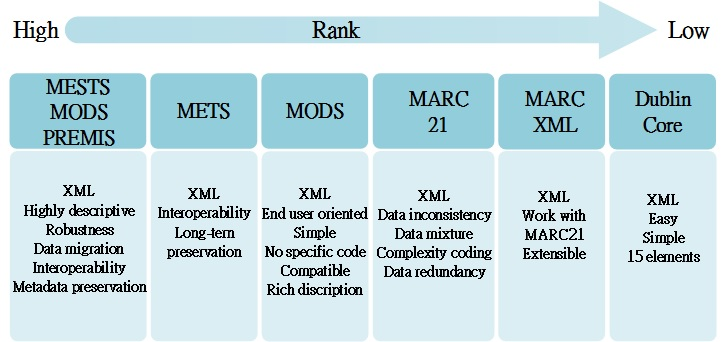
\includegraphics[scale=0.8]{Eagle_unit1}
		\end{center}
		\caption{Overview and hierarchical ranking of Metadata standards and their individual features}
		\vspace{20mm}
		
		

	\end{figure*}
	
	\clearpage % Ends the current page and causes all figures and tables to be printed





